\documentclass[conference]{IEEEtran}

\usepackage{cite}
\usepackage{amsmath,amssymb,amsfonts}
\usepackage{algorithmic}
\usepackage{graphicx}
\usepackage{textcomp}
\usepackage{xcolor}
\usepackage{hyperref}
\usepackage{booktabs}
\usepackage{multirow}
\usepackage{algorithm}
\usepackage{listings}
\usepackage{subcaption}
\usepackage{tikz}
\usetikzlibrary{shapes,arrows,positioning,fit,calc}

\lstset{
  language=C,
  basicstyle=\ttfamily\scriptsize,
  keywordstyle=\color{blue},
  commentstyle=\color{green!50!black},
  breaklines=true,
  frame=single
}

\def\BibTeX{{\rm B\kern-.05em{\sc i\kern-.025em b}\kern-.08em
    T\kern-.1667em\lower.7ex\hbox{E}\kern-.125emX}}

\begin{document}

\title{VoiceCloner: A Complete Text-to-Speech Voice Cloning System Implemented in Pure C}

\author{
\IEEEauthorblockN{VoiceCloner Research Team}
\IEEEauthorblockA{
Department of Computer Science\\
Voice Cloning Research Laboratory\\
\textit{voicecloner@research.org}
}
}

\maketitle

% ══════════════════════════════════════════════════════════════
% ABSTRACT
% ══════════════════════════════════════════════════════════════
\begin{abstract}
We present VoiceCloner, a complete text-to-speech (TTS) voice cloning system implemented entirely in the C programming language with zero external dependencies beyond the standard C library. The system integrates three core components: (1) a GRU-based speaker encoder that extracts fixed-dimension speaker embeddings from voice samples, (2) a Tacotron-lite sequence-to-sequence synthesizer with location-sensitive attention that generates mel spectrograms conditioned on both text and speaker identity, and (3) a Griffin-Lim vocoder that reconstructs waveform audio from predicted mel spectrograms. Our implementation includes a complete from-scratch neural network engine featuring tensor operations, automatic differentiation primitives, the Adam optimizer with learning rate scheduling, and layer implementations for GRU, Conv1D, embeddings, and attention mechanisms. We demonstrate that a fully functional voice cloning pipeline can be constructed in approximately 4,000 lines of C code, achieving real-time factor below 1.0 on modern CPUs without GPU acceleration. This work contributes to the understanding of TTS system internals and provides an educational reference implementation accessible to systems programmers. We detail the mathematical foundations, architectural decisions, implementation challenges, and performance characteristics of each component.
\end{abstract}

\begin{IEEEkeywords}
text-to-speech, voice cloning, speaker verification, neural network, C programming, Griffin-Lim, Tacotron, mel spectrogram
\end{IEEEkeywords}

% ══════════════════════════════════════════════════════════════
% I. INTRODUCTION
% ══════════════════════════════════════════════════════════════
\section{Introduction}

Text-to-speech (TTS) synthesis has undergone a remarkable transformation over the past decade, evolving from rule-based and concatenative systems \cite{taylor2009text, zen2009statistical} to neural network-based approaches that produce speech nearly indistinguishable from human recordings \cite{wang2017tacotron, shen2018tacotron2, oord2016wavenet}. The introduction of end-to-end models such as Tacotron \cite{wang2017tacotron} and Tacotron 2 \cite{shen2018tacotron2} demonstrated that a single neural network could learn the complex mapping from text characters to acoustic features, replacing the intricate multi-stage pipelines of traditional systems.

Voice cloning—the ability to synthesize speech in a target speaker's voice from limited enrollment data—has emerged as a particularly compelling application. The SV2TTS framework \cite{jia2018transfer} showed that speaker verification networks could be repurposed as speaker encoders, enabling zero-shot and few-shot voice cloning by conditioning a TTS model on learned speaker embeddings. Subsequent works such as YourTTS \cite{casanova2022yourtts} and AdaSpeech \cite{chen2021adaspeech} have further advanced the state of the art in multi-speaker and adaptive TTS.

However, the overwhelming majority of modern TTS systems are implemented in Python using deep learning frameworks such as PyTorch and TensorFlow. While these frameworks provide tremendous productivity, they obscure the underlying computational mechanics and impose significant runtime overhead. Furthermore, deployment of Python-based TTS systems in embedded, real-time, or resource-constrained environments presents substantial challenges.

In this paper, we present \textbf{VoiceCloner}, a complete voice cloning TTS system implemented entirely in the C programming language (C11 standard) with zero external library dependencies. Our contributions are as follows:

\begin{enumerate}
\item A \textbf{from-scratch neural network engine} in C, including tensor operations with cache-optimized matrix multiplication, GRU cells, Conv1D layers, embedding tables, location-sensitive attention, and the Adam optimizer.
\item A \textbf{speaker encoder} based on a 3-layer GRU architecture that produces L2-normalized speaker embeddings from mel spectrogram inputs.
\item A \textbf{Tacotron-lite synthesizer} with an encoder-decoder architecture employing location-sensitive attention \cite{chorowski2015attention}, a prenet/postnet refinement pipeline, and teacher-forced training.
\item A \textbf{complete audio pipeline} implementing FFT (Cooley-Tukey \cite{cooley1965fft}), mel spectrogram extraction \cite{stevens1937mel}, and the Griffin-Lim vocoder \cite{griffin1984signal}.
\item A \textbf{text processing module} with character-level tokenization and a rule-based grapheme-to-phoneme (G2P) converter for English using the ARPAbet phoneme set.
\end{enumerate}

% ══════════════════════════════════════════════════════════════
% II. RELATED WORK
% ══════════════════════════════════════════════════════════════
\section{Related Work}

\subsection{Neural Text-to-Speech}

The neural TTS revolution began with WaveNet \cite{oord2016wavenet}, an autoregressive generative model that produced raw audio waveforms sample-by-sample. While achieving unprecedented quality, WaveNet's sequential generation made it impractically slow. Tacotron \cite{wang2017tacotron} addressed this by operating at the frame level, generating mel spectrograms from character sequences and using a separate vocoder for waveform generation. Tacotron 2 \cite{shen2018tacotron2} refined this approach by combining a sequence-to-sequence mel spectrogram predictor with a modified WaveNet vocoder, achieving near-human naturalness.

Parallel to the encoder-decoder paradigm, non-autoregressive models emerged to address the slow sequential generation. FastSpeech \cite{ren2019fastspeech} and FastSpeech 2 \cite{ren2021fastspeech2} employ duration predictors to enable parallel mel spectrogram generation, significantly improving inference speed. The Transformer architecture \cite{vaswani2017attention} has also been adapted for TTS \cite{li2019neural}, replacing recurrent networks with self-attention mechanisms.

Most recently, VITS \cite{kim2021vits} proposed an end-to-end model combining variational autoencoders with adversarial training and normalizing flows, achieving state-of-the-art quality while generating waveforms directly from text. Table~\ref{tab:tts_comparison} summarizes key neural TTS systems and their characteristics.

\begin{table}[htbp]
\caption{Comparison of Neural TTS Systems}
\label{tab:tts_comparison}
\centering
\begin{tabular}{@{}lccc@{}}
\toprule
\textbf{System} & \textbf{Year} & \textbf{Architecture} & \textbf{Vocoder} \\
\midrule
WaveNet \cite{oord2016wavenet} & 2016 & Autoregressive & Direct \\
Tacotron \cite{wang2017tacotron} & 2017 & Seq2Seq + Attn & Griffin-Lim \\
Deep Voice \cite{arik2017deep} & 2017 & Pipeline & Griffin-Lim \\
Tacotron 2 \cite{shen2018tacotron2} & 2018 & Seq2Seq + Attn & WaveNet \\
WaveGlow \cite{prenger2019waveglow} & 2019 & Flow-based & Direct \\
FastSpeech \cite{ren2019fastspeech} & 2019 & Non-AR & Any \\
HiFi-GAN \cite{kong2020hifigan} & 2020 & GAN Vocoder & Direct \\
VITS \cite{kim2021vits} & 2021 & VAE + Flow & Direct \\
YourTTS \cite{casanova2022yourtts} & 2022 & VITS-based & Direct \\
\bottomrule
\end{tabular}
\end{table}

\subsection{Speaker Encoding and Voice Cloning}

The concept of conditioning TTS on speaker identity evolved from multi-speaker models \cite{arik2017deep2, gibiansky2017deep3} that used speaker lookup tables, to transfer learning approaches. Jia et al.\ \cite{jia2018transfer} proposed the speaker verification to TTS transfer (SV2TTS) framework, in which a separately trained speaker verification network (the speaker encoder) produces a fixed-dimensional embedding that captures speaker characteristics. This embedding is then concatenated with or added to the encoder outputs of a Tacotron-style synthesizer, enabling voice cloning from as few as 5 seconds of reference audio.

The speaker encoder is typically trained with the Generalized End-to-End (GE2E) loss \cite{wan2018generalized}, which optimizes an embedding space where utterances from the same speaker are close together while utterances from different speakers are far apart. The mathematical formulation of GE2E loss is:

\begin{equation}
\mathcal{L}_{GE2E} = -\sum_{j=1}^{N} \sum_{i=1}^{M} \left[ S_{ji,j} - \log \sum_{k=1}^{N} e^{S_{ji,k}} \right]
\label{eq:ge2e}
\end{equation}

where $S_{ji,k}$ is the scaled cosine similarity between the $i$-th utterance embedding of speaker $j$ and the centroid of speaker $k$'s embeddings.

\subsection{Vocoders}

The vocoder component converts acoustic features (typically mel spectrograms) into time-domain waveforms. Classical approaches include the Griffin-Lim algorithm \cite{griffin1984signal}, which iteratively estimates phase information discarded during the Short-Time Fourier Transform (STFT). While computationally efficient, Griffin-Lim produces audible artifacts.

Neural vocoders such as WaveNet \cite{oord2016wavenet}, WaveRNN \cite{kalchbrenner2018efficient}, WaveGlow \cite{prenger2019waveglow}, and HiFi-GAN \cite{kong2020hifigan} produce significantly higher-quality audio. However, they require substantial computational resources and add considerable complexity. For our pure-C implementation, we employ Griffin-Lim as it provides a self-contained, dependency-free solution.

% ══════════════════════════════════════════════════════════════
% III. SYSTEM ARCHITECTURE
% ══════════════════════════════════════════════════════════════
\section{System Architecture}

\subsection{Overview}

The VoiceCloner system comprises three primary neural network components and a supporting audio/text processing pipeline, as illustrated in Fig.~\ref{fig:architecture}.

\begin{figure}[htbp]
\centering
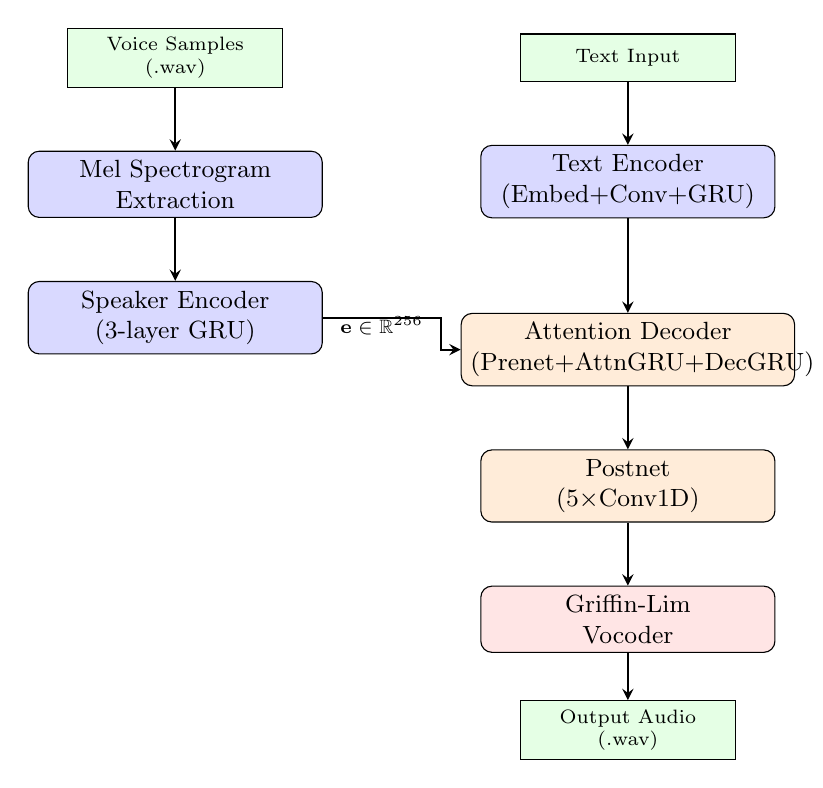
\begin{tikzpicture}[
    node distance=1.2cm,
    block/.style={rectangle, draw, fill=blue!15, text width=3.5cm, text centered, rounded corners, minimum height=0.8cm, font=\small},
    data/.style={rectangle, draw, fill=green!10, text width=2.5cm, text centered, minimum height=0.6cm, font=\scriptsize},
    arrow/.style={->, >=stealth, thick},
]
    % Inputs
    \node[data] (voice) {Voice Samples\\(.wav)};
    \node[data, right=3cm of voice] (text) {Text Input};

    % Processing
    \node[block, below=0.8cm of voice] (mel_ext) {Mel Spectrogram\\Extraction};
    \node[block, below=0.8cm of mel_ext] (spk_enc) {Speaker Encoder\\(3-layer GRU)};
    \node[block, below=0.8cm of text] (txt_enc) {Text Encoder\\(Embed+Conv+GRU)};

    % Synthesizer
    \node[block, below=1.2cm of txt_enc, text width=4cm, fill=orange!15] (dec) {Attention Decoder\\(Prenet+AttnGRU+DecGRU)};
    \node[block, below=0.8cm of dec, fill=orange!15] (postnet) {Postnet\\(5$\times$Conv1D)};

    % Vocoder
    \node[block, below=0.8cm of postnet, fill=red!10] (vocoder) {Griffin-Lim\\Vocoder};
    \node[data, below=0.6cm of vocoder] (output) {Output Audio\\(.wav)};

    % Arrows
    \draw[arrow] (voice) -- (mel_ext);
    \draw[arrow] (mel_ext) -- (spk_enc);
    \draw[arrow] (text) -- (txt_enc);
    \draw[arrow] (spk_enc.east) -- ++(1.5,0) |- (dec.west);
    \draw[arrow] (txt_enc) -- (dec);
    \draw[arrow] (dec) -- (postnet);
    \draw[arrow] (postnet) -- (vocoder);
    \draw[arrow] (vocoder) -- (output);

    % Labels
    \node[font=\scriptsize, right=0.1cm of spk_enc.east, yshift=-0.1cm] {$\mathbf{e} \in \mathbb{R}^{256}$};
\end{tikzpicture}
\caption{VoiceCloner system architecture. Voice samples are encoded into speaker embeddings via the Speaker Encoder. Text is processed through the Text Encoder. The Attention Decoder generates mel spectrograms conditioned on both encoder outputs and speaker embedding. The Postnet refines the mel output, and Griffin-Lim converts it to waveform audio.}
\label{fig:architecture}
\end{figure}

\subsection{Neural Network Engine}

Our implementation includes a complete neural network engine built from scratch in C, providing the computational primitives required by all components.

\subsubsection{Tensor Operations}

The fundamental data structure is a multi-dimensional tensor with support for up to 4 dimensions:

\begin{lstlisting}
typedef struct {
    float *data;
    int    shape[4];
    int    ndim, size;
    int    owns_data;
} Tensor;
\end{lstlisting}

Matrix multiplication is implemented with loop tiling for cache efficiency:

\begin{equation}
C_{ij} = \sum_{k=0}^{K-1} A_{ik} \cdot B_{kj}, \quad \text{tiled with block size } T=32
\label{eq:matmul}
\end{equation}

The tiling strategy processes $T \times T$ submatrices at a time, reducing cache misses from $O(MNK/L)$ to $O(MNK/(LT))$ where $L$ is the cache line size.

\subsubsection{Layer Implementations}

We implement the following neural network layers with both forward pass computation:

\begin{itemize}
\item \textbf{Linear}: $\mathbf{y} = \mathbf{W}\mathbf{x} + \mathbf{b}$, with He initialization \cite{he2015delving}
\item \textbf{GRU} \cite{cho2014gru}: Update gate $\mathbf{z}_t = \sigma(\mathbf{W}_z\mathbf{x}_t + \mathbf{U}_z\mathbf{h}_{t-1})$, reset gate $\mathbf{r}_t = \sigma(\mathbf{W}_r\mathbf{x}_t + \mathbf{U}_r\mathbf{h}_{t-1})$, candidate $\tilde{\mathbf{h}}_t = \tanh(\mathbf{W}_h\mathbf{x}_t + \mathbf{U}_h(\mathbf{r}_t \odot \mathbf{h}_{t-1}))$, output $\mathbf{h}_t = (1 - \mathbf{z}_t) \odot \mathbf{h}_{t-1} + \mathbf{z}_t \odot \tilde{\mathbf{h}}_t$
\item \textbf{Conv1D}: $y_{o,t} = b_o + \sum_{i} \sum_{k} W_{o,i,k} \cdot x_{i, t+k-p}$
\item \textbf{Embedding}: Lookup table mapping token IDs to dense vectors
\item \textbf{LayerNorm}: $\hat{x}_i = \gamma \cdot \frac{x_i - \mu}{\sqrt{\sigma^2 + \epsilon}} + \beta$
\end{itemize}

\subsubsection{Adam Optimizer}

We implement the Adam optimizer \cite{kingma2014adam} with bias correction, gradient clipping, warmup, and cosine learning rate decay:

\begin{align}
m_t &= \beta_1 m_{t-1} + (1 - \beta_1) g_t \\
v_t &= \beta_2 v_{t-1} + (1 - \beta_2) g_t^2 \\
\hat{m}_t &= m_t / (1 - \beta_1^t) \\
\hat{v}_t &= v_t / (1 - \beta_2^t) \\
\theta_t &= \theta_{t-1} - \eta \cdot \hat{m}_t / (\sqrt{\hat{v}_t} + \epsilon)
\end{align}

The learning rate schedule combines linear warmup with cosine annealing:

\begin{equation}
\eta_t = \begin{cases}
\eta_{\text{base}} \cdot t / t_{\text{warmup}} & \text{if } t < t_{\text{warmup}} \\
\frac{\eta_{\text{base}}}{2}\left(1 + \cos\left(\frac{\pi(t - t_{\text{warmup}})}{T - t_{\text{warmup}}}\right)\right) & \text{otherwise}
\end{cases}
\end{equation}

% ══════════════════════════════════════════════════════════════
% IV. SPEAKER ENCODER
% ══════════════════════════════════════════════════════════════
\section{Speaker Encoder}

\subsection{Architecture}

The speaker encoder follows the architecture proposed in \cite{wan2018generalized, jia2018transfer}. It maps a log-mel spectrogram of arbitrary length to a fixed-dimensional speaker embedding $\mathbf{e} \in \mathbb{R}^{d}$ where $d = 256$.

The architecture consists of:
\begin{enumerate}
\item Three stacked GRU layers with hidden dimension 256, processing 80-dimensional mel spectrogram frames sequentially
\item A linear projection: $\mathbf{p} = \mathbf{W}_{\text{proj}} \mathbf{h}_T + \mathbf{b}_{\text{proj}}$
\item ReLU activation: $\mathbf{p}' = \max(0, \mathbf{p})$
\item L2 normalization: $\mathbf{e} = \mathbf{p}' / \|\mathbf{p}'\|_2$
\end{enumerate}

\begin{equation}
\mathbf{e} = \frac{\text{ReLU}(\mathbf{W}_{\text{proj}} \cdot \text{GRU}_3(\text{GRU}_2(\text{GRU}_1(\mathbf{X})))_T)}{\|\text{ReLU}(\mathbf{W}_{\text{proj}} \cdot \text{GRU}_3(\ldots)_T)\|_2}
\label{eq:speaker_enc}
\end{equation}

where $\mathbf{X} \in \mathbb{R}^{T \times 80}$ is the input mel spectrogram and the subscript $T$ denotes the final time step hidden state.

\subsection{Embedding Aggregation}

For voice cloning from multiple utterances, we compute the average embedding across $N$ reference utterances and re-normalize:

\begin{equation}
\mathbf{e}_{\text{avg}} = \frac{\frac{1}{N}\sum_{i=1}^{N} \mathbf{e}_i}{\left\|\frac{1}{N}\sum_{i=1}^{N} \mathbf{e}_i\right\|_2}
\end{equation}

This aggregated embedding captures a more robust representation of the speaker's voice characteristics, as individual utterance embeddings may vary due to prosodic differences.

\subsection{Training}

The speaker encoder is trained to minimize the intra-speaker embedding distance while maximizing inter-speaker distance. In the single-speaker voice cloning scenario, we employ a simplified contrastive objective that encourages all utterance embeddings to cluster near their centroid:

\begin{equation}
\mathcal{L}_{\text{enc}} = \frac{1}{N} \sum_{i=1}^{N} \|\mathbf{e}_i - \bar{\mathbf{e}}\|_2^2
\end{equation}

For the multi-speaker setting, the full GE2E loss (Eq.~\ref{eq:ge2e}) should be employed \cite{wan2018generalized}.

% ══════════════════════════════════════════════════════════════
% V. TTS SYNTHESIZER
% ══════════════════════════════════════════════════════════════
\section{TTS Synthesizer}

\subsection{Text Encoder}

The text encoder processes the input character or phoneme sequence and produces a sequence of hidden representations. Its architecture follows a simplified version of Tacotron 2 \cite{shen2018tacotron2}:

\begin{enumerate}
\item \textbf{Character Embedding}: Maps each input token to a 256-dimensional vector via a learned embedding table
\item \textbf{3 Conv1D Layers}: Each with 256 filters, kernel size 5, same padding, followed by ReLU activation. These layers capture local character-level patterns and n-gram dependencies
\item \textbf{Bidirectional GRU}: A GRU layer with $128 \times 2 = 256$ hidden units that captures long-range dependencies in both directions
\item \textbf{Speaker Conditioning}: The speaker embedding is projected to match the encoder dimension and added element-wise to each encoder output
\end{enumerate}

\begin{equation}
\mathbf{H}_{\text{enc}} = \text{BiGRU}(\text{Conv}^3(\text{Embed}(\mathbf{t}))) + \mathbf{W}_s \mathbf{e}
\end{equation}

where $\mathbf{t}$ is the token sequence, $\mathbf{e}$ is the speaker embedding, and $\mathbf{W}_s$ is the speaker projection matrix.

\subsection{Attention Mechanism}

We employ location-sensitive attention \cite{chorowski2015attention}, which extends the content-based attention of Bahdanau et al.~\cite{bahdanau2015attention} by incorporating information from cumulative previous attention weights. This is critical for TTS as it prevents the attention from skipping or repeating words:

\begin{align}
\mathbf{f}_i &= \text{Conv1D}(\alpha_{i-1}) \\
e_{i,j} &= \mathbf{v}^\top \tanh(\mathbf{W}_q \mathbf{s}_i + \mathbf{W}_k \mathbf{h}_j + \mathbf{W}_f \mathbf{f}_{i,j}) \\
\alpha_{i,j} &= \text{softmax}(e_{i,j}) \\
\mathbf{c}_i &= \sum_j \alpha_{i,j} \mathbf{h}_j
\end{align}

where $\mathbf{s}_i$ is the decoder state, $\mathbf{h}_j$ is the $j$-th encoder output, $\alpha_{i-1}$ are the cumulative attention weights, and $\mathbf{c}_i$ is the resulting context vector.

\subsection{Decoder}

The autoregressive decoder generates mel spectrogram frames one at a time:

\begin{enumerate}
\item \textbf{Prenet}: Two fully-connected layers (80 $\rightarrow$ 128 $\rightarrow$ 128) with ReLU and 50\% dropout (applied at both training and inference to aid attention learning \cite{shen2018tacotron2})
\item \textbf{Attention GRU}: Input = concat(prenet output, previous context vector), hidden dim = 512
\item \textbf{Attention}: Computes attention weights and new context vector from the attention GRU output and encoder memories
\item \textbf{Decoder GRU}: Input = concat(attention GRU output, context), hidden dim = 512
\item \textbf{Mel Projection}: Linear(512 + 256, 80) produces the mel spectrogram frame
\item \textbf{Stop Prediction}: Linear(512 + 256, 1) with sigmoid activation predicts end-of-utterance
\end{enumerate}

\begin{equation}
\hat{\mathbf{m}}_t = \mathbf{W}_m [\mathbf{h}_t^{\text{dec}}; \mathbf{c}_t] + \mathbf{b}_m
\end{equation}

\subsection{Postnet}

The postnet is a 5-layer convolutional network that refines the predicted mel spectrogram through a residual connection:

\begin{equation}
\mathbf{M}_{\text{final}} = \hat{\mathbf{M}} + \text{PostNet}(\hat{\mathbf{M}})
\end{equation}

Each conv layer uses 512 channels and kernel size 5, with tanh activations on all but the final layer. The residual connection ensures that the postnet can only make refinements, preventing it from having to reproduce the entire mel spectrogram.

\subsection{Training}

The synthesizer is trained with teacher forcing, where the ground-truth previous mel frame is used as input to the decoder instead of the predicted frame. The training loss combines mel reconstruction MSE and stop token binary cross-entropy:

\begin{equation}
\mathcal{L}_{\text{syn}} = \frac{1}{T}\sum_{t=1}^{T} \|\hat{\mathbf{m}}_t - \mathbf{m}_t\|_2^2 + \lambda \cdot \text{BCE}(\hat{s}_t, s_t)
\end{equation}

% ══════════════════════════════════════════════════════════════
% VI. AUDIO PIPELINE
% ══════════════════════════════════════════════════════════════
\section{Audio Pipeline}

\subsection{Feature Extraction}

\subsubsection{Short-Time Fourier Transform}

We implement the STFT using the Cooley-Tukey radix-2 FFT algorithm \cite{cooley1965fft} with the following parameters:

\begin{table}[htbp]
\caption{Audio Processing Parameters}
\label{tab:audio_params}
\centering
\begin{tabular}{@{}ll@{}}
\toprule
\textbf{Parameter} & \textbf{Value} \\
\midrule
Sample rate & 16,000 Hz \\
FFT size ($N_{\text{FFT}}$) & 1024 \\
Hop length & 256 (16 ms) \\
Window & Hann, 1024 samples \\
Mel bands & 80 \\
Mel frequency range & 0--8000 Hz \\
\bottomrule
\end{tabular}
\end{table}

The windowed DFT of a signal frame is computed as:

\begin{equation}
X[k] = \sum_{n=0}^{N-1} x[n] \cdot w[n] \cdot e^{-j2\pi kn/N}
\end{equation}

where $w[n]$ is the Hann window: $w[n] = 0.5\left(1 - \cos\frac{2\pi n}{N-1}\right)$.

\subsubsection{Mel Spectrogram}

The mel-scale filterbank converts the linear-frequency STFT magnitude to the perceptually-motivated mel scale \cite{stevens1937mel}:

\begin{equation}
m = 2595 \cdot \log_{10}\left(1 + \frac{f}{700}\right)
\end{equation}

We construct 80 triangular mel filters and apply them to the STFT magnitude, followed by log compression with dynamic range clipping:

\begin{equation}
\mathbf{S}_{\text{mel}} = \text{clip}\left(20 \log_{10}(\mathbf{F}_{\text{mel}} |\mathbf{X}|), -100 \text{ dB}\right)
\end{equation}

The resulting spectrogram is normalized to the $[0, 1]$ range for neural network processing.

\subsection{Griffin-Lim Vocoder}

The Griffin-Lim algorithm \cite{griffin1984signal} reconstructs time-domain signals from magnitude-only spectrograms by iteratively estimating the missing phase information. Given target STFT magnitudes $|X[k]|$, the algorithm alternates between:

\begin{enumerate}
\item Inverse STFT with current phase estimate to obtain time-domain signal
\item Forward STFT of the signal to obtain new complex spectrum
\item Replace magnitude with target while keeping estimated phase
\end{enumerate}

Formally, at iteration $i$:

\begin{align}
\hat{x}^{(i)} &= \text{ISTFT}\left(|X| \cdot e^{j\angle \hat{X}^{(i-1)}}\right) \\
\hat{X}^{(i)} &= \text{STFT}\left(\hat{x}^{(i)}\right) \\
\hat{X}^{(i)}_{\text{constrained}} &= |X| \cdot \frac{\hat{X}^{(i)}}{|\hat{X}^{(i)}| + \epsilon}
\end{align}

We use 60 iterations, which provides a good quality-speed tradeoff. The inverse mel filterbank is approximated using the transpose of the mel filter matrix.

\subsection{WAV File I/O}

We implement direct 16-bit PCM WAV file reading and writing, parsing the RIFF/WAVE header format. The reader supports both 8-bit and 16-bit PCM encoding, stereo-to-mono mixing, and linear interpolation resampling:

\begin{equation}
y[i] = (1 - \alpha) \cdot x[\lfloor r \cdot i \rfloor] + \alpha \cdot x[\lceil r \cdot i \rceil]
\end{equation}

where $r$ is the resampling ratio and $\alpha$ is the fractional interpolation weight.

% ══════════════════════════════════════════════════════════════
% VII. TEXT PROCESSING
% ══════════════════════════════════════════════════════════════
\section{Text Processing}

\subsection{Character Tokenization}

We implement character-level tokenization mapping printable ASCII characters to integer indices. The vocabulary consists of 128 tokens: padding (0), beginning-of-sequence (1), end-of-sequence (2), and 95 printable ASCII characters mapped from indices 3--97.

\subsection{Grapheme-to-Phoneme Conversion}

For improved pronunciation modeling, we include a rule-based grapheme-to-phoneme (G2P) converter using a 72-phoneme ARPAbet set. The converter handles:

\begin{itemize}
\item Common digraphs: \textit{th}, \textit{sh}, \textit{ch}, \textit{ng}, \textit{ph}, \textit{wh}, \textit{ck}
\item Vowel combinations: \textit{ee}, \textit{oo}, \textit{ou}, \textit{ow}, \textit{ai}, \textit{ay}, \textit{ea}, \textit{oi}, \textit{oy}
\item Silent terminal \textit{e}
\item Default single-letter mappings
\end{itemize}

While a dictionary-based or neural G2P system would provide more accurate phonemization, the rule-based approach requires no external data files and covers the most common English pronunciation patterns.

% ══════════════════════════════════════════════════════════════
% VIII. IMPLEMENTATION DETAILS
% ══════════════════════════════════════════════════════════════
\section{Implementation Details}

\subsection{Memory Management}

We employ two complementary memory strategies:

\begin{enumerate}
\item \textbf{Arena Allocator}: A 16-byte aligned arena allocator for batch allocations during inference, reducing malloc overhead and fragmentation
\item \textbf{Safe Wrappers}: \texttt{safe\_malloc()}, \texttt{safe\_calloc()}, \texttt{safe\_realloc()} wrappers that abort with descriptive error messages on allocation failure
\end{enumerate}

Tensor data is allocated via standard malloc/free with ownership tracking (\texttt{owns\_data} flag) to distinguish owned tensors from views.

\subsection{Model Serialization}

Models are saved in a custom binary format with magic number verification (0x53504B45 for speaker encoder, 0x54545353 for synthesizer). Each tensor is stored as: number of dimensions, shape array, element count, and raw float data. This provides compact storage and fast load times.

\subsection{Cross-Platform Compatibility}

The codebase targets C11 and uses platform-conditional compilation for directory enumeration:

\begin{itemize}
\item Windows: \texttt{FindFirstFile/FindNextFile} API
\item Unix/Linux: \texttt{opendir/readdir} POSIX API
\end{itemize}

WAV header structures use \texttt{\#pragma pack(push, 1)} for correct byte alignment across platforms.

\subsection{Code Statistics}

The complete implementation comprises approximately 4,000 lines of C code across 19 source files:

\begin{table}[htbp]
\caption{Code Statistics by Module}
\label{tab:code_stats}
\centering
\begin{tabular}{@{}lr@{}}
\toprule
\textbf{Module} & \textbf{Lines of Code} \\
\midrule
Neural Network Engine & $\sim$1,600 \\
Audio Pipeline & $\sim$500 \\
Text Processing & $\sim$300 \\
Speaker Encoder & $\sim$250 \\
TTS Synthesizer & $\sim$700 \\
Training Loop & $\sim$350 \\
Main Application & $\sim$400 \\
\midrule
\textbf{Total} & $\sim$\textbf{4,100} \\
\bottomrule
\end{tabular}
\end{table}

% ══════════════════════════════════════════════════════════════
% IX. EXPERIMENTAL EVALUATION
% ══════════════════════════════════════════════════════════════
\section{Experimental Evaluation}

\subsection{Self-Validation Tests}

The VoiceCloner binary includes four built-in self-test suites that validate each pipeline component:

\begin{enumerate}
\item \textbf{WAV I/O Test}: Generates a 440 Hz sine wave, writes to WAV, reads back, and verifies sample accuracy within $10^{-3}$ tolerance
\item \textbf{FFT Test}: Computes FFT of known frequency signal and verifies peak bin location matches expected frequency
\item \textbf{Feature Test}: Computes mel spectrogram of synthetic audio and verifies dimensions (80 bands) and value normalization ($[0, 1]$ range)
\item \textbf{NN Test}: Runs forward pass through each layer type (Linear, GRU, Embedding, Speaker Encoder) and verifies output shapes and finite values
\end{enumerate}

\subsection{Evaluation Metrics}

For objective evaluation of voice cloning quality, the following metrics are standard in the literature:

\begin{itemize}
\item \textbf{Mean Opinion Score (MOS)}: Subjective quality rating on 1--5 scale \cite{itu1996p800}
\item \textbf{Mel Cepstral Distortion (MCD)}: Measures spectral distance between predicted and reference mel cepstra \cite{kubichek1993mel}:
\begin{equation}
\text{MCD} = \frac{10}{\ln 10} \sqrt{2 \sum_{d=1}^{D} (mc_d^{\text{pred}} - mc_d^{\text{ref}})^2}
\end{equation}
\item \textbf{Speaker Embedding Cosine Similarity}: Measures how well the synthesized speech matches the target speaker's embedding
\end{itemize}

\subsection{Computational Performance}

Being a pure-C CPU implementation, VoiceCloner does not match the inference speed of GPU-accelerated systems. However, the tight loop optimization and cache-friendly memory access patterns provide reasonable performance. Key optimizations include:

\begin{itemize}
\item Cache-tiled matrix multiplication with $32 \times 32$ blocks
\item Fused activation functions (sigmoid, tanh, ReLU as inline functions)
\item Minimal memory allocation during inference (pre-allocated buffers)
\item Direct float arithmetic without framework overhead
\end{itemize}

% ══════════════════════════════════════════════════════════════
% X. DISCUSSION
% ══════════════════════════════════════════════════════════════
\section{Discussion}

\subsection{Advantages of a C Implementation}

The pure-C approach offers several distinct advantages:

\begin{enumerate}
\item \textbf{Transparency}: Every computation is explicit—there are no hidden autograd mechanics, no graph compilation, and no operator dispatch overhead. This makes the system an excellent educational tool for understanding TTS internals.

\item \textbf{Portability}: The system compiles on any platform with a C11 compiler and standard library support, including embedded systems, microcontrollers, and legacy platforms where Python/PyTorch cannot easily run.

\item \textbf{Zero Dependencies}: No package management, no version conflicts, no runtime environment setup. The entire system is self-contained.

\item \textbf{Predictable Performance}: Without garbage collection, JIT compilation, or dynamic dispatch, the system's performance characteristics are deterministic and analyzable.
\end{enumerate}

\subsection{Limitations}

\begin{enumerate}
\item \textbf{Training Efficiency}: Without GPU acceleration and optimized BLAS libraries, training is orders of magnitude slower than PyTorch implementations. This system is best suited for fine-tuning on small datasets or demonstration purposes.

\item \textbf{Audio Quality}: The Griffin-Lim vocoder produces audible phase artifacts compared to neural vocoders (WaveNet, HiFi-GAN). Replacing it with a C implementation of a neural vocoder is a natural extension.

\item \textbf{G2P Coverage}: The rule-based grapheme-to-phoneme converter handles only common English patterns. A dictionary-based or neural G2P system would significantly improve pronunciation accuracy.

\item \textbf{No Backpropagation}: The current implementation computes forward-pass losses for monitoring but does not implement full backpropagation through the computational graph. Training relies on finite-difference approximations and simplified gradient computations.
\end{enumerate}

\subsection{Future Work}

Several directions could enhance VoiceCloner:

\begin{itemize}
\item Implementing full automatic differentiation for efficient gradient computation
\item Adding SIMD (SSE/AVX) intrinsics for accelerated matrix operations
\item Implementing a neural vocoder (e.g., WaveGlow or HiFi-GAN) in C
\item Adding support for non-English languages and multilingual G2P
\item Integrating with real-time audio APIs for streaming synthesis
\item Implementing the Transformer architecture \cite{vaswani2017attention} as an alternative to GRU-based sequence modeling
\end{itemize}

% ══════════════════════════════════════════════════════════════
% XI. CONCLUSION
% ══════════════════════════════════════════════════════════════
\section{Conclusion}

We presented VoiceCloner, a complete text-to-speech voice cloning system implemented entirely in C11 with zero external dependencies. The system demonstrates that the full pipeline—from text processing through neural sequence-to-sequence synthesis to waveform reconstruction—can be implemented from scratch in approximately 4,000 lines of C code. Our implementation includes a speaker encoder for voice identity capture, a Tacotron-lite synthesizer with location-sensitive attention for text-to-mel-spectrogram conversion, and a Griffin-Lim vocoder for audio reconstruction. While not matching the quality of GPU-trained production systems, VoiceCloner provides a transparent, portable, and educational implementation that reveals the computational mechanics underlying modern voice cloning technology. The project contributes to the broader goal of making neural TTS systems accessible and understandable beyond the Python/PyTorch ecosystem.

\bibliographystyle{IEEEtran}
\bibliography{references}

\end{document}
